\documentclass[12pt]{article}
\usepackage[a4paper, top=2.5cm, bottom=2.5cm, left=1.5cm, right=1.5cm]{geometry}
\usepackage{amsmath, amsfonts, amssymb, mathtools}
\usepackage{fancyhdr, setspace, parskip}
\usepackage{graphicx, caption, subfig, array, multirow}
\usepackage{hyperref, enumitem, cancel}
\usepackage[T1]{fontenc}
\usepackage{tgtermes}
\usepackage[dvipsnames]{xcolor}
\usepackage{tocloft}
\usepackage{titlesec}
\usepackage{lipsum}  

\definecolor{DarkBlue}{RGB}{10, 0, 80}

% Hyperlink setup
\hypersetup{
    colorlinks=true,
    linkcolor=DarkBlue,
    filecolor=BrickRed,      
    urlcolor=RoyalBlue,
}


% Header and footer customization
\fancyhead{}
\fancyhead[L]{
{\fontfamily{lmss}{\color{DarkBlue}
\textbf{\leftmark}
}}
}
\fancyhead[R]{
{\fontfamily{ppl}\selectfont {\color{DarkBlue}
{Deep RL Course [Spring 2025]}
}}
}

\fancyfoot{}
\fancyfoot[C]{
{\fontfamily{lmss}{\color{BrickRed}
\textbf{\thepage}
}}
}

\renewcommand{\sectionmark}[1]{ \markboth{\thesection\quad #1}{} }

\renewcommand{\headrule}{{\color{BrickRed}\hrule width\headwidth height 0.5pt}}
\renewcommand{\footrulewidth}{0pt}


% Table of Contents customizations
\renewcommand{\cftsecafterpnum}{\vskip6pt}
\renewcommand{\cftsubsecafterpnum}{\vskip3pt}
\renewcommand{\cftsubsubsecafterpnum}{\vskip3pt}
\renewcommand{\cftsecfont}{\sffamily\large}
\renewcommand{\cftsubsecfont}{\sffamily}
\renewcommand{\cftsubsubsecfont}{\sffamily}
% \renewcommand{\cftsecdotsep}{1}
\renewcommand{\cftsubsecdotsep}{1}
\renewcommand{\cftsubsubsecdotsep}{1}


% Section title styles
\titleformat*{\section}{\LARGE\bfseries\color{DarkBlue}}
\titleformat*{\subsection}{\Large\bfseries\color{DarkBlue}}
\titleformat*{\subsubsection}{\large\bfseries\color{DarkBlue}}

\definecolor{light-gray}{gray}{0.95}
\newcommand{\code}[1]{\colorbox{light-gray}{\texttt{#1}}}

% Start of the document
\pagestyle{fancy}

%%%%%%%%%%%%%%%%%%%%%%%%%%%%%%%%%%%%%%%%%%%%%%%%%

\begin{document}

\pagenumbering{gobble}
\thispagestyle{plain}

\begin{center}

\vspace*{-1.5cm}
\begin{figure}[!h]
    \centering
    
\includegraphics[width=0.7\linewidth]{figs/cover-std.png}
\end{figure}

{
\fontfamily{ppl}

{\color{DarkBlue} {\fontsize{30}{50} \textbf{
Deep Reinforcement Learning
}}}

{\color{DarkBlue} {\Large
Professor Mohammad Hossein Rohban
}}
}


\vspace{20pt}

{
\fontfamily{lmss}

{\color{RedOrange}
{\Large
Solution for Homework 13:
}\\
}
{\color{BrickRed}
\rule{12cm}{0.5pt}

{\Huge
Multi-Agent RL

}
\rule{12cm}{0.5pt}
}

\vspace{10pt}

{\color{RoyalPurple} { \small By:} } \\
\vspace{10pt}

{\color{Blue} { \LARGE [Full Name] } } \\
\vspace{5pt}
{\color{RoyalBlue} { \Large [Student Number] } }


\vspace*{\fill}
\begin{center}
\begin{tabular}{ccc}
    
\includegraphics[width=0.14\linewidth]{figs/sharif-logo.png} & 
\includegraphics[width=0.14\linewidth]{figs/riml-logo.png} & 
\includegraphics[width=0.14\linewidth]{figs/dlr-logo.png} \\
\end{tabular}
\end{center}


\vspace*{-.25cm}

{\color{YellowOrange} {
\rule{10cm}{0.5pt} \\
\vspace{2pt}
\large Spring 2025}
}}
\vspace*{-1cm}

\end{center}

%%%%%%%%%%%%%%%%%%%%%%%%%%%%%%%%%%%%%%%%%%%%%%%%%

\newpage
\pagenumbering{gobble}

{\fontfamily{lmss}\selectfont {\color{DarkBlue}

\subsection*{Grading}

The grading will be based on the following criteria, with a total of 110 points:

\[
\begin{array}{|l|l|}
\hline
\textbf{Task} & \textbf{Points} \\
\hline
\text{Task 1} & 50 \\
\text{Task 2} & 50 \\

\hline
\text{Clarity and Quality of Code} & 5 \\
\text{Clarity and Quality of Report} & 5 \\
\hline
\text{Bonus 1} & 5 \\
\text{Bonus 2} & 5 \\
\hline
\end{array}
\]


%%%%%%%%%%%%%%%%%%%%%%%%%%%%%%%%%%%%%%%%%%%%%%%%%

\newpage
\thispagestyle{plain}
{\fontfamily{lmss}\selectfont {\color{BrickRed} \textbf{\tableofcontents} }}


%%%%%%%%%%%%%%%%%%%%%%%%%%%%%%%%%%%%%%%%%%%%%%%%%

\newpage
\pagenumbering{arabic}

{\fontfamily{lmss}\selectfont {\color{DarkBlue}



\section{Part 1: Game Theory Problems}





%%%%%%%%%%%%%%%%%%%%%%%%%%%%%%%%%%%%%%%%%%%%%%%%%

\newpage

{\fontfamily{lmss}\selectfont {\color{DarkBlue}

\section{Part 2: Implementing MADDPG/IDDPG}

\begin{enumerate}
    \item In our training loop, the \texttt{DDPGLoss} module utilizes \texttt{target\_policies} to estimate the value of the next state. Explain clearly why employing these slowly-updating target networks, rather than the main policy networks (which change rapidly), is essential for ensuring the stability of the DDPG algorithm. (Hint: Consider what might happen if the critic tried to optimize toward a continuously moving target.)

    \item (bonus) Consider the training plot shown in Figure~\ref{fig:unstable_learning}, which resulted from modifying a single scalar hyper-parameter in the training script.
    \begin{enumerate}
        \item Describe the issue with the learning process depicted in the plot.
        \item Identify which hyper-parameter you believe was changed, and explain the role of this parameter within the MADDPG algorithm.
    \end{enumerate}
\end{enumerate}

\begin{figure}[h!]
    \centering
    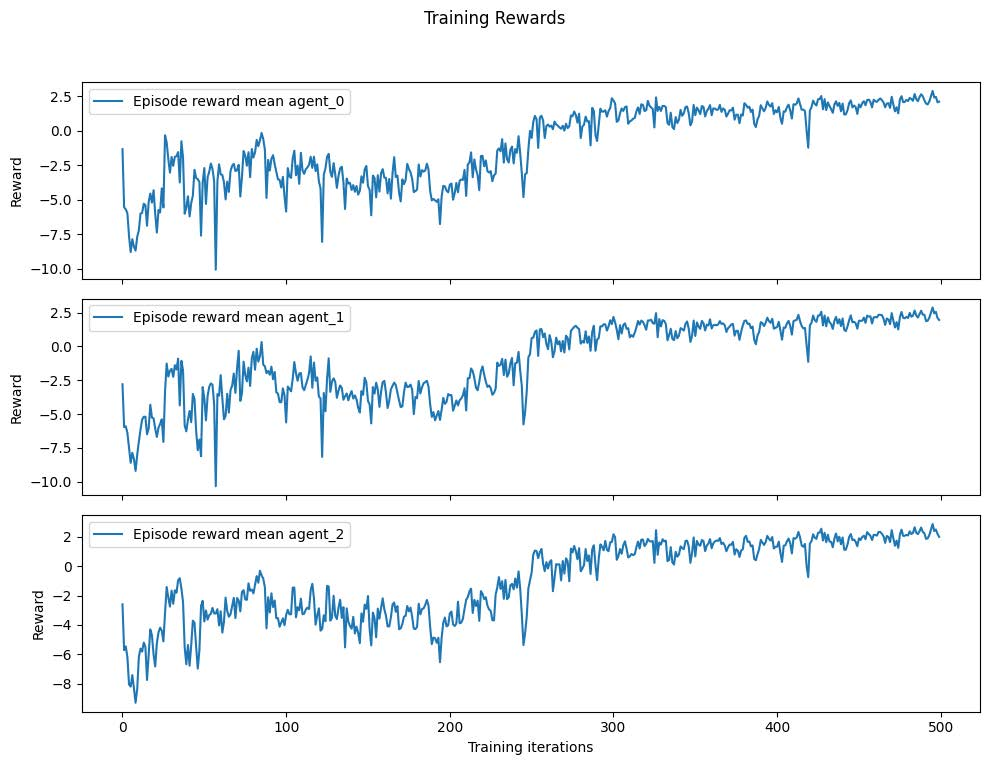
\includegraphics[width=0.75\linewidth]{figs/results.jpg}
    \caption{Agents performance after modifying a scalar hyper-parameter.}
    \label{fig:unstable_learning}
\end{figure}




}}


%%%%%%%%%%%%%%%%%%%%%%%%%%%%%%%%%%%%%%%%%%%%%%%%%

\newpage

{\fontfamily{lmss}\selectfont {\color{DarkBlue}

\begin{thebibliography}{9}

\bibitem{Freepik}
\href{https://www.freepik.com/free-vector/cute-artificial-intelligence-robot-isometric-icon_16717130.htm}{Cover image designed by freepik}

\bibitem{lowe2017multi}
Ryan Lowe, Yi I. Wu, Aviv Tamar, Jean Harb, Pieter Abbeel, and Igor Mordatch.
\newblock Multi-agent actor-critic for mixed cooperative-competitive environments.
\newblock In \emph{Advances in Neural Information Processing Systems (NeurIPS)}, 2017.
\newblock \href{https://arxiv.org/abs/1706.02275}{arXiv:1706.02275}


\end{thebibliography}


}}

%%%%%%%%%%%%%%%%%%%%%%%%%%%%%%%%%%%%%%%%%%%%%%%%%

\end{document}